GPU memory use grows strictly linearly with respect to the number of streams and threads. When going from one to two streams, bwa-gasal2 takes twice as much memory. In this section, we will present the case we deemed more representative of real use.

GPU memory (VRAM) use is a delicate topic to assess, since it highly depends on various factors:

\begin{itemize}
	\item the GPU, since the VRAM available may not be sufficient to saturate its computing resources,
	\item the CPU, because how many threads we can instantiate directly impacts how much VRAM we will need,
	\item the RAM, since the sequences also need to be loaded in RAM before being copied to the GPU (although this is rarely a limiting factor, since a given machine usually has far more RAM than its GPU has VRAM),
	\item and of course, the data set running.
\end{itemize}

We cannot conduct measurements that are corresponding to any algorithmic truth in this case. Consequently we will present the memory use as a case study corresponding to our current machine and data sets, and we will see if, in our example case, the memory use can be deemed as reasonable. We consider the GPU we used (Tesla K40c) with its 2880 CUDA cores and its 12GB or VRAM, as representative of the accelerators generally used.

For this, we start bwa-gasal2 with a substantial low amount of memory, and let the automatic memory extension grow until the end of the program. The memory use for data set SRR150 and SRR250 is shown on Figure~\ref{fig:memory-use}. We measured memory use for what we consider a regular use case for our machine : 12 threads, with 2 streams. 

\begin{figure}[h]
	\centering
	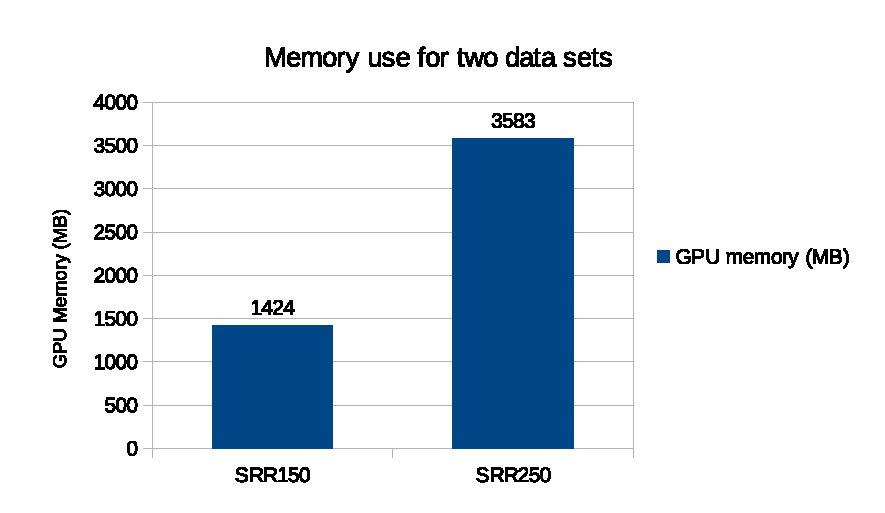
\includegraphics[width=0.9\linewidth]{memory-use}
	\caption{Memory use for our two data sets on our testing machine}
	\label{fig:memory-use}
\end{figure}

In these tests, we need around 1570 MB for a data set with sequences of 150 bases, and 2730 MB for sequences 250 bases long. We use less than 1/6th of our total available memory with our worst case scenario. In particular, this allows to use a low VRAM accelerator if needed. Moreover,it leaves more memory to accelerate other parts of the application.

We also measure the SM utilisation in percents with the utilitary \verb|nvidia-smi|. We log this utilisation during the program execution with a resolution of one measure per second. Results are available for data set SRR150 for 1 an 2 streams on Figure~\ref{fig:sm-use-srr150-1str} and Figure~\ref{fig:sm-use-srr150-2str}.

\begin{figure}[h]
	\centering
	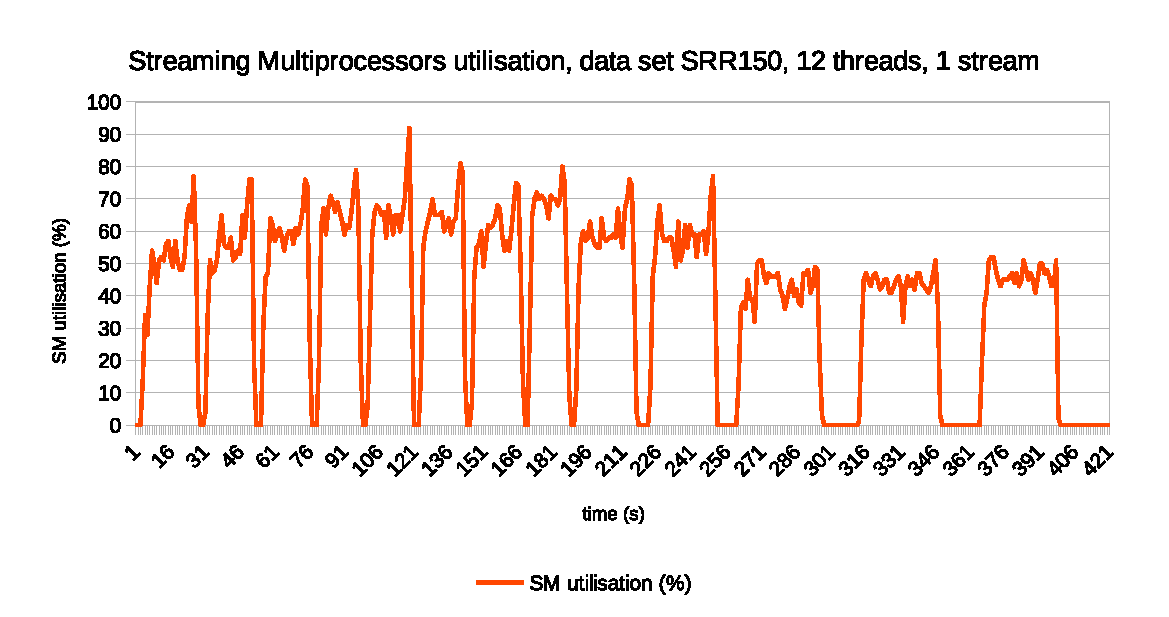
\includegraphics[width=0.9\linewidth]{SM_utilisation_12threads1stream}
	\caption{SM use for SRR150 with 1 stream on our testing machine}
	\label{fig:sm-use-srr150-1str}
\end{figure}

\begin{figure}[h]
	\centering
	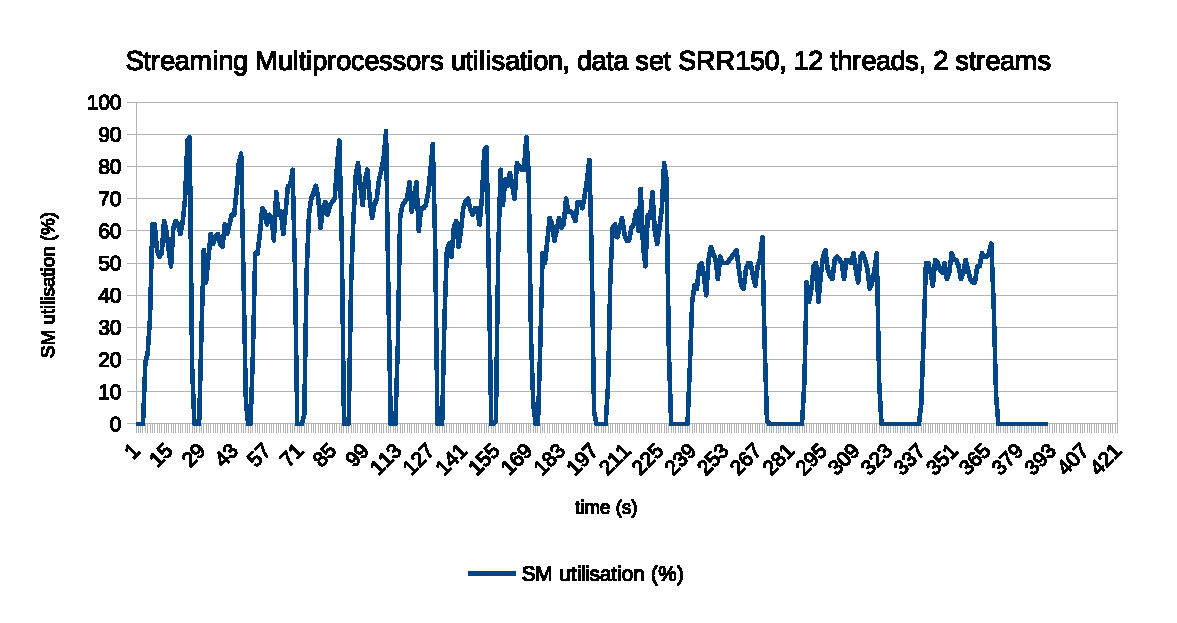
\includegraphics[width=0.9\linewidth]{SM_utilisation_12threads2streams}
	\caption{SM use for SRR150 with 2 streams on our testing machine}
	\label{fig:sm-use-srr150-2str}
\end{figure}

We can notice several interesting points:
\begin{itemize}
    \item SM use fluctuates noticeably when the GPU is actively used. While the mean is around 70\%, some peaks to 90\% are present. Our GPU is not completely used, but we already take the major part of its computing resources.
    \item Globally, the GPU stays active most of the time, so we are efficiently using its computing power.
    \item SM utilisation is a bit lower with a single stream, which is logical: with two streams, the GPU may have to compute both data sets at the same time when they overlap, which leads to a higher SM use. Still, with 2 streams, the SM use is by no means the double of when we use 1 stream: streams are rarely overlapping, meaning that using 2 streams allows to use the resources more efficiently without saturating the GPU.
    \item During the mapping, the GPU can be idle for a short period of time. Depending on the data it has to process, it can be one second (in the beginning) up to 5 seconds (at the end). These idle periods are moments where the CPU is still running the seeding part. There is room to accelerate another part, for example seeding, on the GPU: this could bring us close to saturation of the computing cores.
\end{itemize}{}

In the case of data set SRR250, results are available for one stream in Figure~\ref{fig:sm-use-srr250-1str} and for two streams in Figure~\ref{fig:sm-use-srr250-2str}.

\begin{figure}[h]
	\centering
	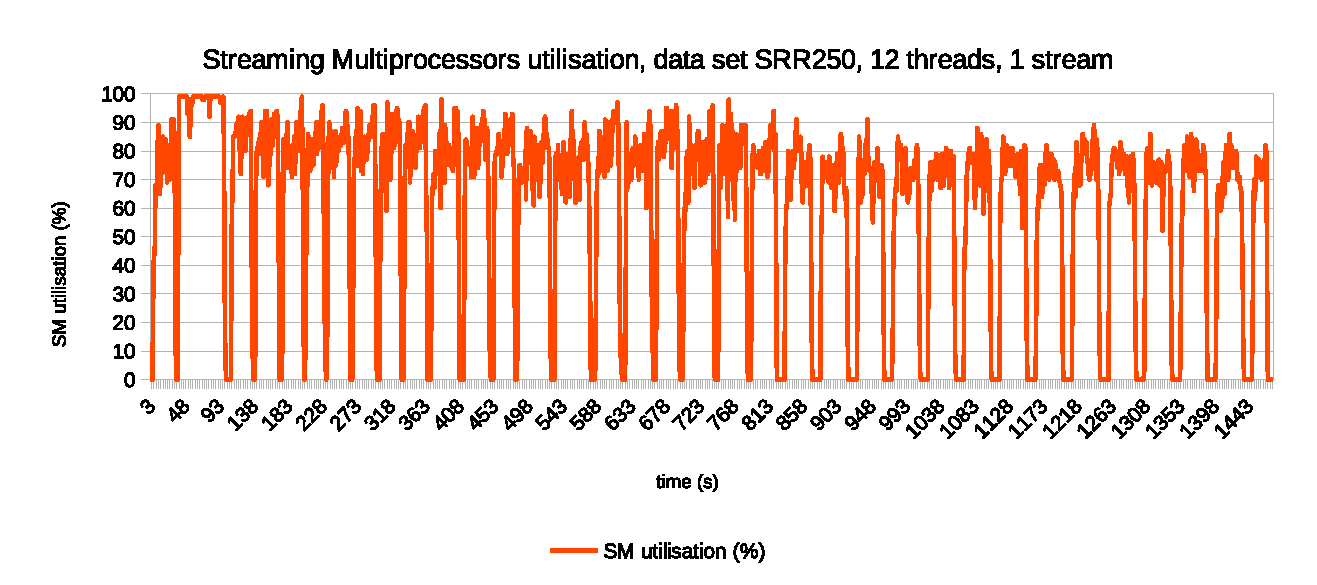
\includegraphics[width=0.9\linewidth]{SM_utilisation_12threads1stream_SRR250}
	\caption{SM use for SRR250 with 1 stream on our testing machine}
	\label{fig:sm-use-srr250-1str}
\end{figure}

\begin{figure}[h]
	\centering
	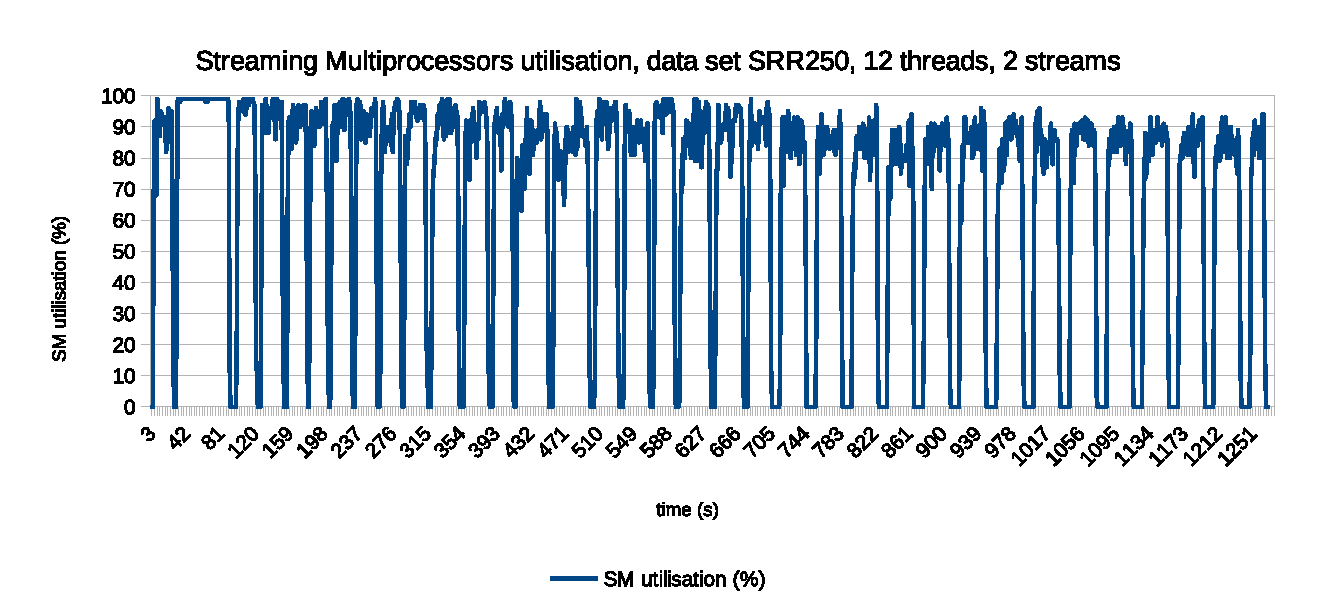
\includegraphics[width=0.9\linewidth]{SM_utilisation_12threads2streams_SRR250}
	\caption{SM use for SRR250 with 2 streams on our testing machine}
	\label{fig:sm-use-srr250-2str}
\end{figure}

For this data set, the GPU is noticeably more active, as the SM utilisation is most of the time above 80\%. With two streams, it even reaches 100\% use many times. Still, there are the same moments where the GPU goes idle for up to several seconds. These moments could still beneficiate